\documentclass[a4paper,11pt]{article}

\usepackage[T1]{fontenc}
\usepackage[french]{babel}
\usepackage{graphicx}
\usepackage{lmodern}
\usepackage[utf8]{inputenc}
\usepackage{parskip}
\usepackage{tikz}
\usetikzlibrary{arrows.meta, positioning}
\usepackage{float}
\usepackage[margin=2.5cm]{geometry}

\usepackage{listings}
\usepackage{xcolor}
\usepackage{textcomp}
\usepackage{upquote}

% Configuration du style
\lstset{
    language=Java,
    basicstyle=\ttfamily\small,
    backgroundcolor=\color{black!5},
    keywordstyle=\color{blue}\bfseries,
    stringstyle=\color{purple},
    commentstyle=\color{green!60!black}\itshape,
    numbers=none,
    rulecolor=\color{black!30},
    frame=single,
    breaklines=true,
    columns=fullflexible,
    keepspaces=true,
    showstringspaces=false,
    showspaces=false,
    upquote=true,
    extendedchars=true,
    morekeywords={String, System, Thread, Runnable, Exception, RuntimeException, Object},
    literate=
    {é}{{\'e}}1
    {è}{{\`e}}1
    {ê}{{\^e}}1
    {à}{{\`a}}1
    {â}{{\^a}}1
    {ç}{{\c{c}}}1
    {ù}{{\`u}}1
    {î}{{\^i}}1
    {ô}{{\^o}}1
    {'}{\textquotesingle}1
}

%Info document
\title{Rapport Projet - Programmation répartie}
\author{Alexis CERDA DE ALMEIDA VILACA\\ Logan SAGET \\Taïno HERMANN \\ Emelyne FOUSSE}
\date{\today}

\begin{document}

\maketitle
\tableofcontents
\newpage

% ===================================================
\section{Introduction}
% ===================================================

\textit{Lien du répertoire GIT :} \texttt{https://github.com/HermannT88/projet\_rmi\_calcul\_parallele}

Pour 

\newpage

% ===================================================
\section{Le raytracer local}
% ===================================================

\subsection{Mesures de temps d'exécution}

Pour réalisés des mesures sur le temps de calcul, nous avons fait une boucle qui exécute 10 fois le calcul de l'image avec à chaque itération \texttt{largeur = i * largeur de base} et \texttt{hauteur = i * hauteur de base}

\begin{lstlisting}
for (int i = 1; i<= 10; i++ ){
  int l = largeur*i, h = hauteur*i;
  
  Instant debut = Instant.now();
  System.out.println("Itération " + i + " Largeur = " + l + "Hauteur = "+ h);
  Image image = scene.compute(x0, y0, l, h);
  Instant fin = Instant.now();

  long duree = Duration.between(debut, fin).toMillis();
            
  System.out.println("Temps de calcul :"+duree+" ms");
}
\end{lstlisting}

Nous obtenons alors ces résultats :

\begin{table}[H]
\centering
\begin{tabular}{|c|c|c|c|}
\hline
\textbf{Itération} & \textbf{Largeur (px)} & \textbf{Hauteur (px)} & \textbf{Temps de calcul (ms)} \\
\hline
1 & 512 & 512 & 3182 \\
\hline
2 & 1024 & 1024 & 7372 \\
\hline
3 & 1536 & 1536 & 13642 \\
\hline
4 & 2048 & 2048 & 23977 \\
\hline
5 & 2560 & 2560 & 32773 \\
\hline
6 & 3072 & 3072 & 48813 \\
\hline
7 & 3584 & 3584 & 64370 \\
\hline
8 & 4096 & 4096 & 84049 \\
\hline
9 & 4608 & 4608 & 107256 \\
\hline
10 & 5120 & 5120 & 128906 \\
\hline
\end{tabular}
\caption{Évolution du temps de calcul en fonction des dimensions}
\end{table}

\vspace{0.5cm}
\begin{figure}[H]
  \noindent
  \begin{center}
  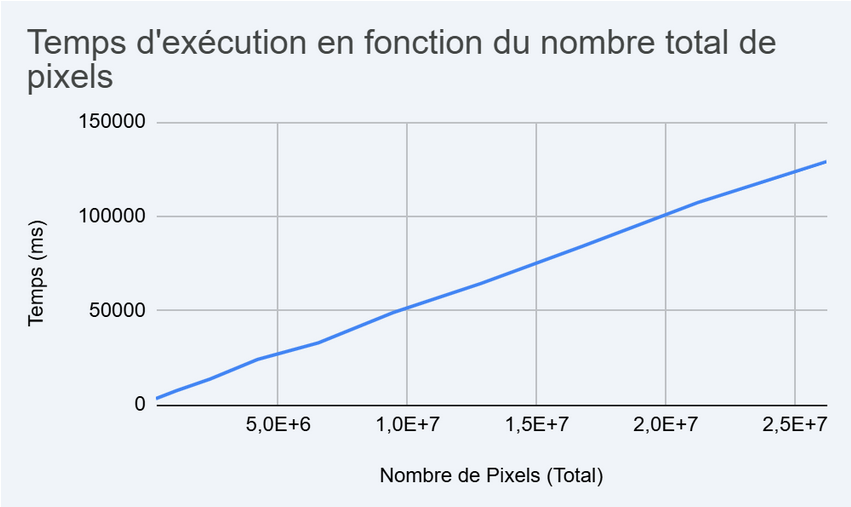
\includegraphics[width=\textwidth]{images/courbe.png}
  \end{center}
  \caption{\underline{Temps d'éxecution en fonction des pixels}}
\end{figure}
\vspace{0.5cm}

Nous constatons que le temps de calcul augmente proportionnelement au nombre de pixels de l'image.

\subsection{Reproduction de l'image}

L'objectif est de reproduire l'image ci-dessous :

\begin{figure}[H]
  \noindent
  \begin{center}
  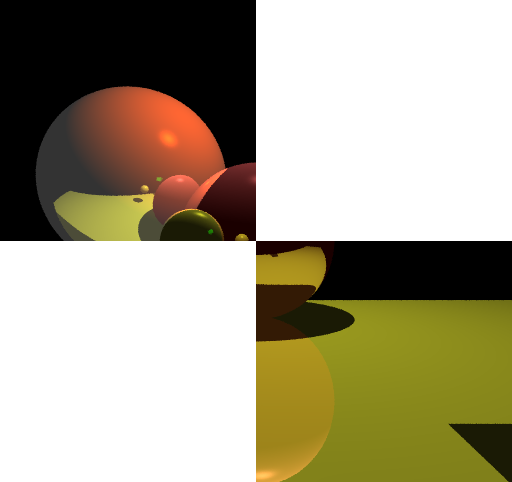
\includegraphics[width=7cm]{images/raytrace-resultat-2.png}
  \end{center}
  \caption{\underline{Image à reproduire}}
\end{figure}
\vspace{0.5cm}



Pour reproduire l'image, nous allons calculer individuellement les deux parties de l'image attendue.

La première partie, le programme va calculer l'image en partant des coordonnées 0 ; 0 soit le coin supérieur droit. Puis il va calculer l'image jusqu'a son centre, donc à la moitier de la hauteur et la moitier de la largeur. Ce qui nous donne la ligne suivante :

\begin{lstlisting}
  Image image1 = scene.compute(x0, y0, l/2, h/2);
\end{lstlisting}

Pour la seconde, nous allons recréé une image qui cette fois va commencer au millieu et encore avancé en largeur et en hauteur de la moitié. Nous avons alors cette ligne :

\begin{lstlisting}
  Image image2 = scene.compute(l/2, h/2, l/2, h/2);
\end{lstlisting}

Enfin nous affichons les deux images calculée précédemment sur la même fenêtre, avec la première au coordonnées 0 ; 0 et la seconde au centre de l'image :

\begin{lstlisting}
  disp.setImage(image1, x0, y0);
  disp.setImage(image2, l/2, h/2);
\end{lstlisting}

Pour le code complet, nous arrivons donc à ce résultat :

\begin{lstlisting}
int x0 = 0, y0 = 0;
int l = largeur, h = hauteur;

// Chronométrage du temps de calcul
Instant debut = Instant.now();
System.out.println("Calcul de l'image :\n - Coordonnées : "+x0+","+y0
+"\n - Taille "+ largeur + "x" + hauteur);
Image image1 = scene.compute(x0, y0, l/2, h/2);
Image image2 = scene.compute(l/2, h/2, l/2, h/2);
Instant fin = Instant.now();

long duree = Duration.between(debut, fin).toMillis();

System.out.println("Image calculée en :"+duree+" ms");

// Affichage de l'image calculée
disp.setImage(image1, x0, y0);
disp.setImage(image2, l/2, h/2);
\end{lstlisting}

\newpage

% ===================================================
\section{Architecture de l'application répartie}
% ===================================================

\subsection{Schéma de l'architecture}

Pour notre première idée d'architecture, l'application avait un client qui envoyait le fichier txt correspondant à l'image à calculer au service central. Ce service se serait ensuite chargé du découpage en threads et de la répartition entre les nœuds de calcul. Une fois l'image calculée entièrement, le service central aurait renvoyé l'objet Image au Client.

\begin{figure}[H]
  \noindent
  \begin{center}
  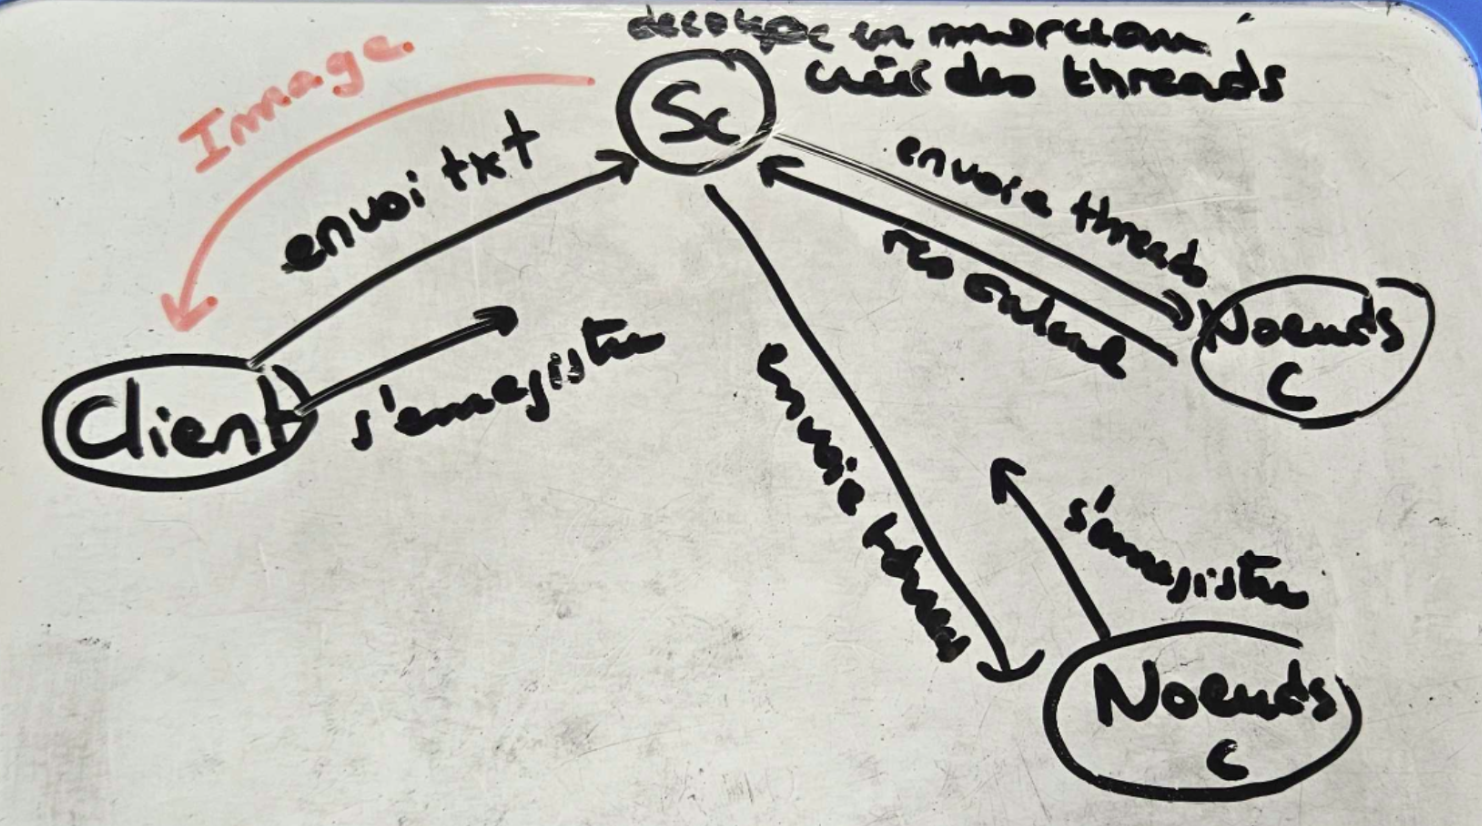
\includegraphics[width=12cm]{images/shema1.png}
  \end{center}
  \caption{\underline{Première version}}
\end{figure}
\vspace{0.5cm}

Pour la deuxième version, le fonctionnement était très similaire à la première version, avec cette fois toute la partie découpage des tâches et échanges avec les nœuds déléguée à un service Répartiteur.

\begin{figure}[H]
  \noindent
  \begin{center}
  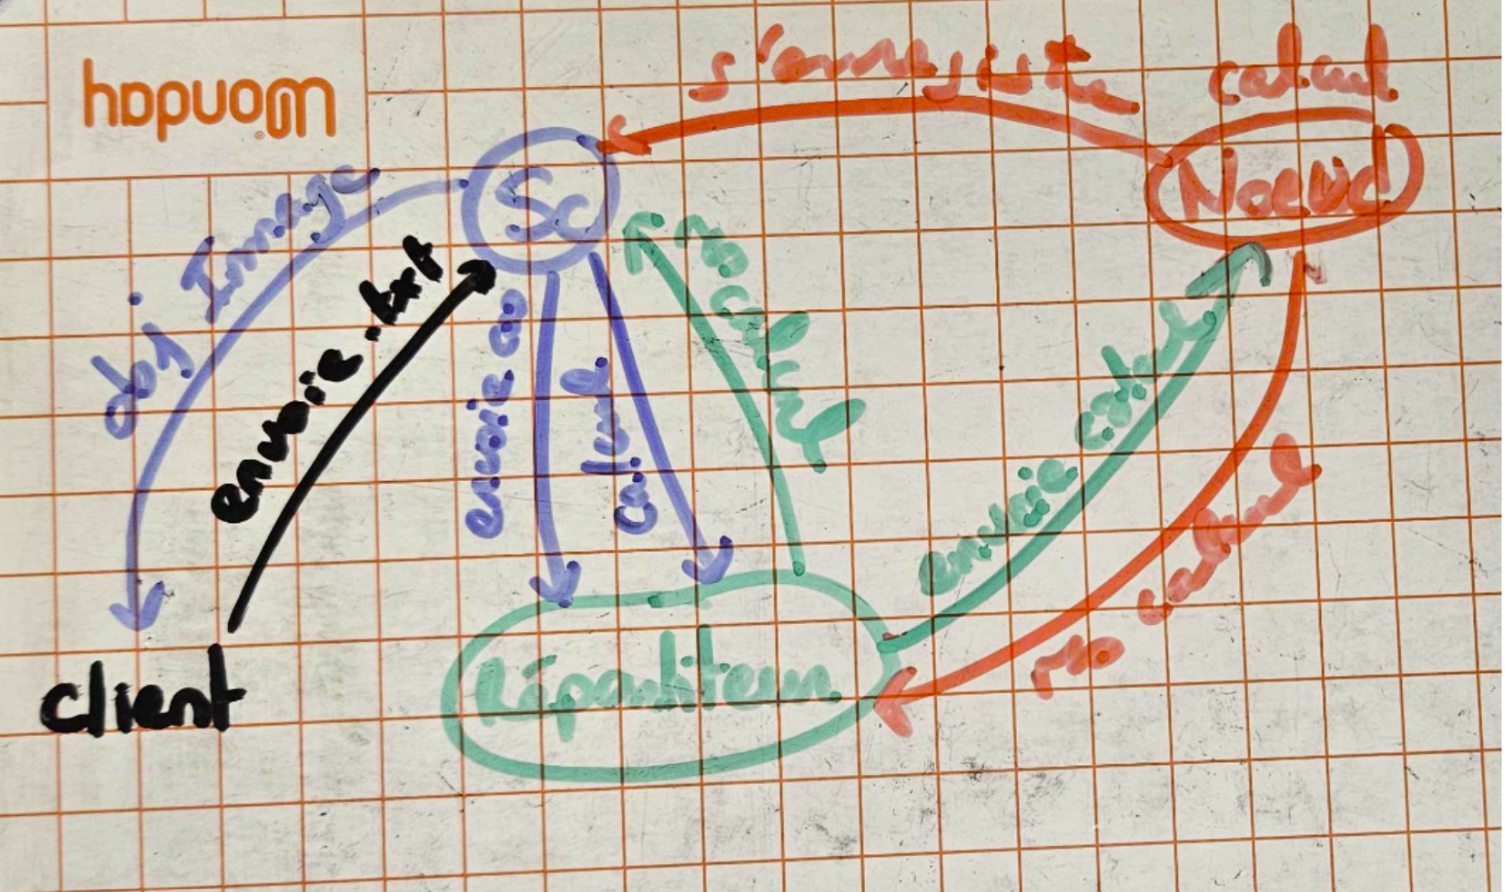
\includegraphics[width=12cm]{images/shema2.png}
  \end{center}
  \caption{\underline{Deuxième version}}
\end{figure}
\vspace{0.5cm}

Dans la version finale, toute la logique de découpage en threads a été redonnée au Client. Le service central ne sert plus qu'à fournir et gérer les nœuds, c'est-à-dire maintenir une liste de nœuds, en ajouter, en supprimer et envoyer un nœud lorsqu'un Client le demande.

\begin{figure}[H]
  \noindent
  \begin{center}
  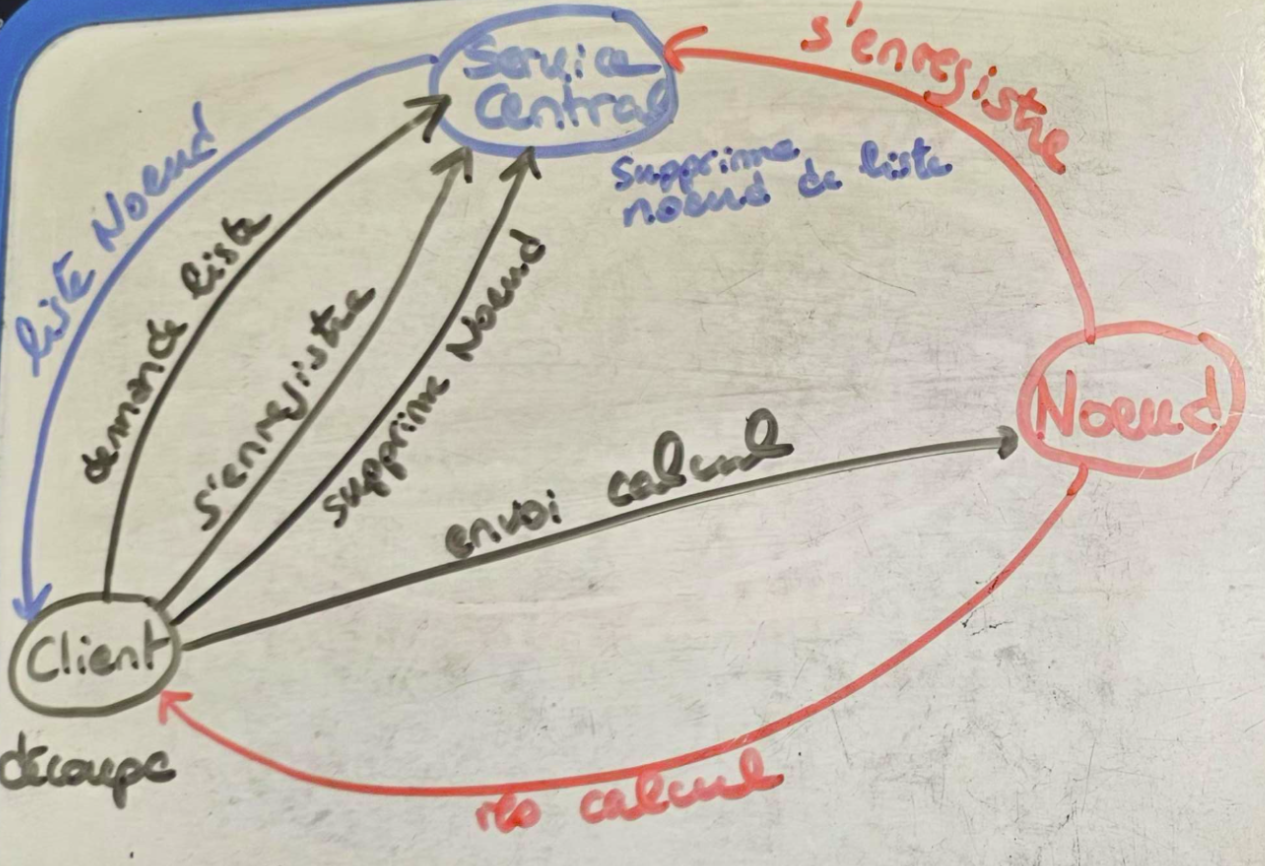
\includegraphics[width=12cm]{images/shema3.png}
  \end{center}
  \caption{\underline{Version finale}}
\end{figure}
\vspace{0.5cm}

* Contrairement à ce qui est indiqué sur le schéma, le service central renvoie un unique nœud au client et non la liste entière.

\subsection{Processus fixes et processus mobiles}

Les processus mobiles sont représentés par les différents nœuds de calculs qui peuvent s'enregistrer et se déconnecter. On peut également considérer le client qui est à l'origine de la demande de calcul comme un processus mobile.

Le processus fixe est le service qui va transmettre le calcul aux différents noeuds de calculs. Le service est enregistré sur un port.

\subsection{Données échangées entre les processus}

Le client envoie un fichier .txt et les coordonnées relatives à la création de l'image (deux pour le point initial et deux pour la longueur et la largeur des pixels). Il reçoit un objet "Image" une fois celle-ci construite.

Une fois ces calculs réalisés, les noeuds retournent le résultat et le service central va l'interpréter.

\newpage

% ===================================================
\section{Fonctionnement des composants}
% ===================================================

\subsection{Le service central}

% TODO

\subsection{Les nœuds de calcul}

% TODO

\subsection{Le client / dispatcher}

% TODO

\newpage

% ===================================================
\section{Mise en œuvre du parallélisme}
% ===================================================

\subsection{Distribution des tâches en threads}



\subsection{Synchronisation et assemblage des résultats}

% TODO

\newpage

% ===================================================
\section{Conclusion}
% ===================================================

% TODO

\end{document}